%%%%%%%%%%%%%%%%%%%%%%%%%%%%%%%%%%%%%%%%%12pt: grandezza carattere
                                        %a4paper: formato a4
                                        %openright: apre i capitoli a destra
                                        %twoside: serve per fare un
                                        %   documento fronteretro
                                        %report: stile tesi (oppure book)
\documentclass[12pt,a4paper,openright,twoside]{report}
%\usepackage[english]{babel}
\usepackage[english]{babel}
\usepackage[latin1]{inputenc}
\usepackage{fancyhdr}
\usepackage{indentfirst}
\usepackage{graphicx}
\usepackage{newlfont}
\usepackage{amssymb}
\usepackage{amsmath}
\usepackage{latexsym}
\usepackage{amsthm}
\usepackage{hyperref}
\usepackage{listings}

\oddsidemargin=30pt \evensidemargin=20pt%impostano i margini
\hyphenation{sil-la-ba-zio-ne pa-ren-te-si}%serve per la sillabazione: tra parentesi 
					   %vanno inserite come nell'esempio le parole 
%					   %che latex non riesce a tagliare nel modo giusto andando a capo.

%
%%%%%%%%%%%%%%%%%%%%%%%%%%%%%%%%%%%%%%%%%comandi per l'impostazione
                                        %   della pagina, vedi il manuale
                                        %   della libreria fancyhdr
                                        %   per ulteriori delucidazioni
\pagestyle{fancy}\addtolength{\headwidth}{20pt}
\renewcommand{\chaptermark}[1]{\markboth{\thechapter.\ #1}{}}
\renewcommand{\sectionmark}[1]{\markright{\thesection \ #1}{}}
\rhead[\fancyplain{}{\bfseries\leftmark}]{\fancyplain{}{\bfseries\thepage}}
\cfoot{}
%%%%%%%%%%%%%%%%%%%%%%%%%%%%%%%%%%%%%%%%%
\linespread{1} % era 1.3                %comando per impostare l'interlinea
%%%%%%%%%%%%%%%%%%%%%%%%%%%%%%%%%%%%%%%%%definisce nuovi comandi
%
\begin{document}
\begin{titlepage}

\begin{center}
{{\Large{\textsc{Alma Mater Studiorum $\cdot$ Universit\`a di
Bologna}}}} \rule[0.1cm]{15.8cm}{0.1mm}
\rule[0.5cm]{15.8cm}{0.6mm}
{\small{\bf SCUOLA DI SCIENZE\\
Corso di Laurea Magistrale in Informatica }}
\end{center}
\vspace{15mm}
\begin{center}
{\LARGE{\bf TITOLO}}\\
\vspace{3mm}
{\LARGE{\bf DELLA}}\\
\vspace{3mm}
{\LARGE{\bf TESI}}\\
\end{center}
\vspace{40mm}
\par
\noindent
\begin{minipage}[t]{0.47\textwidth}
{\large{\bf Relatore:\\
Chiar.mo Prof.\\
Renzo Davoli}}
\end{minipage}
\hfill
\begin{minipage}[t]{0.47\textwidth}\raggedleft
{\large{\bf Presentata da:\\
Mattia Maldini}}
\end{minipage}
\vspace{20mm}
\begin{center}
{\large{\bf Sessione III\\%inserire il numero della sessione in cui ci si laurea
Anno Accademico 2018-2019}}%inserire l'anno accademico a cui si � iscritti
\end{center}
%
\newpage                                %va in una pagina nuova
\thispagestyle{empty}                   %elimina il numero della pagina
\topmargin=6.5cm                        %imposta il margina superiore a 6.5cm
\raggedleft                             %incolonna la scrittura a destra
\large                                  %aumenta la grandezza del carattere
                                        %   a 14pt
\em                                     %emfatizza (corsivo) il carattere
Questa \`e la \textsc{Dedica}:\\
ognuno pu\`o scrivere quello che vuole, \\
anche nulla \ldots                      %\ldots lascia tre puntini
\newpage                                %va in una pagina nuova



\clearpage{\pagestyle{empty}\cleardoublepage}%non numera l'ultima pagina sinistra
\end{titlepage}
\pagenumbering{roman}                   %serve per mettere i numeri romani
\chapter*{Abstract}                 %crea l'introduzione (un capitolo
                                        %   non numerato)
The course of Operative Systems is arguably one of the most crucial part of 
a computer science course. While it is safe to say a small minority of students
will ever face the challenge to develop software below the OS level, the 
understanding of its principles is paramount in the formation of a proper computer
scientist.
The theory behind operative systems is not a particularly complex topic. Ideas 
like process scheduling, execution levels and resource semaphores are intuitively
grasped by students; yet mastering these notions thorugh abstract study alone
will prove tedious if not impossible. 

Devising a practical - albeit simplified - implementation of said notions can
go a long way in helping students to really understand the underlying workflow
of the processor as a whole in all its nuances. 

Developing a proof-of-concept OS, however, is not as simple as creating software for
an already existing one. The complexity of real-world hardware
 goes way beyond what students are required to learn, which makes hard to
 find a proper machine architecture to run the project on.

This work is heavily inspired by uMPS2 (and uARM), a previous solution to this problem:
 an emulator for the MPIS R3000 processor. By working on a virtual and simplified
 version of the hardware many of the unnecessary tangles are stripped away while
 still mantaining the core concepts of OS development.
Although inspired by a real architecture (MIPS), uMPS2 is still an abstract 
environment; this allows the students' work to be controlled and directed,
 but might leave some of them with a feeling of detachment from reality
 (as was the case for the author).

What is argued in this thesis is that a similar project can be developed
on real hardware without becoming too complicated. The designed architecture
is ARMv8, more modern and widespread, in the form of the Raspberry Pi education
board.

The result of this work is dual: on one side there was a thorough study on
how to develop a basic OS on the Raspberry Pi 3, a knowledge that is
as of now not properly documented for those not prepared on the topic; using
this knowledge an hardware abstraction layer has been developed for 
initialization and usage of various hardware peripherals, allowing users
to buid a toy OS on top of it.
While the final product can be used without knowing how it works internally 
(in a similar fashion to the $\mu$MPS) emulator, all the code was written 
trying to remain as simple and clear as possible to encourage a deeper study
as example.

\clearpage{\pagestyle{empty}\cleardoublepage}%non numera l'ultima pagina sinistra
\chapter*{Sommario}
TODO: traduzione dell'abstract

%%%%%%%%%%%%%%%%%%%%%%%%%%%%%%%%%%%%%%%%%non numera l'ultima pagina sinistra
\clearpage{\pagestyle{empty}\cleardoublepage}
\tableofcontents                        %crea l'indice
%%%%%%%%%%%%%%%%%%%%%%%%%%%%%%%%%%%%%%%%%imposta l'intestazione di pagina
\rhead[\fancyplain{}{\bfseries\leftmark}]{\fancyplain{}{\bfseries\thepage}}
\lhead[\fancyplain{}{\bfseries\thepage}]{\fancyplain{}{\bfseries
INDICE}}
%%%%%%%%%%%%%%%%%%%%%%%%%%%%%%%%%%%%%%%%%non numera l'ultima pagina sinistra
\clearpage{\pagestyle{empty}\cleardoublepage}
\listoffigures                          %crea l'elenco delle figure
%%%%%%%%%%%%%%%%%%%%%%%%%%%%%%%%%%%%%%%%%non numera l'ultima pagina sinistra
\clearpage{\pagestyle{empty}\cleardoublepage}
\listoftables                           %crea l'elenco delle tabelle
%%%%%%%%%%%%%%%%%%%%%%%%%%%%%%%%%%%%%%%%%non numera l'ultima pagina sinistra
\clearpage{\pagestyle{empty}\cleardoublepage}
\chapter{Introduction}                %crea il capitolo
%%%%%%%%%%%%%%%%%%%%%%%%%%%%%%%%%%%%%%%%%imposta l'intestazione di pagina
\lhead[\fancyplain{}{\bfseries\thepage}]{\fancyplain{}{\bfseries\rightmark}}
\pagenumbering{arabic}                  %mette i numeri arabi
\section{Background}
An operative system is, in a nutshell, a very complex and sophisticated program
that manages the resources of its host machine. Proper studying on the topic 
should yield higher understanding on many fields of the likes of
parallel programming, concurrency, data structures, security and 
code management in general.

As previously mentioned, an Operating Systems course should ideally include
field work. This can be done through several different approaches, which
have already been covered by previous works like $\mu$ARM and $\mu$MPS
\cite{tesijonjic} \cite{tesimelletti}.
To quickly recap the most notable mentions:
\begin{description}
    \item[Study of an existing OS] the most theoretical approach, it involves
        reading and analyzing the source code. There is no short supply of such
        examples; historically Minix is cited \cite{minix}, but a quick research
        will reveal countless small kernels for embedded platforms and emulators.
        The biggest downside to this approach is that the esamination of the source
        code may end up not having more educational value than a pseudocode snippet
        found in the textbook. The fact that the example is indeed practical is 
        lost in the lack of application by the student.
    \item[Modification of an existing OS] this approach can be seen as a slight
        revision to the study-only policy. If the work under examination can indeed
        be run in some environment, students might find themselves modifying small
        parts even if unprompted by the professor.
    \item[Construction from scratch] this is the idea behind projects $\mu$MPS, 
        $\mu$MPS2, $\mu$ARM and the KayaOS specification \cite{davolimorsiani}.
\end{description}

It is argued that the last approach is the most interesting and valuable for 
the students. If they are to study an existing Operative System at all, it is
either the case that said OS would be too complex or simple enough for them 
to implement. In the first scenario the studying program must skip the most cumbersome
parts and only cover what is essential, in which case the completeness 
of the example loses meaning. In the latter there is no reason not to follow 
the constructionist route and let the disciples create their own OS.

\subsection{$\mu$MPS and Similar Emulators}
Every learning project must find a balance between abstraction and concreteness.
Developing a real world application with value outside of the academic context
 brings the most satisfaction to the scholar; frequently, however, an entirely
 practical assignment would lose a lot of learning value due to hindrances
 spanning outside of the course program.
 
In the frame of this work said hindrances would be the complexities tied to
hardware architecture of peripherals and CPU that, although interesting
int their own right, are unnecessary for the students' formation process.
The $\mu$MPS emulator provides an environment fairly similar to real hardware
while still being approchable for an undergraduate student; it positions itself
in a sweet spot between abstraction and concreteness, allowing just enough
of the underlying hardware to pass through and keeping the focus on 
theoretical topics like memory management, scheduling and concurrency.

After successfully concluding his or her work on $\mu$MPS the student has
a firm grasp on said topics and has grown significantly in the ability to
manage large and complex projects. There can be, however, a lingering confusion
on the attained result, which is limited to a relatively small niche.
The software itself may be compiled for a real architecture, but the final binary
can only run on the simplified emulator, making it a trial for its own sake.

The final end of $\mu$MPS is, in fact, learning, so this is not really a shortcoming.
What is attemped with this work is to take a small step towards concreteness in 
the aforementioned balance without falling into a pit of unnecessary complexity.
The occasion to do so is presented by the rise of a widespread and relatively
clean architecture: ARMv8, specifically using the Raspberry Pi 3 educational board.

\subsection{ARMv8 and Raspberry Pi}
The passage from MIPSEL to ARM is not new to $\mu$MPS; the previous work
of $\mu$ARM was already pointed in this direction. $\mu$ARM had the goal to
modernize the $\mu$MPS experience, thus maintaing its emulator-only approach.
In fact, when this work started the goal was to create an hardware abstraction
layer to be able to run an $\mu$ARM project on Raspberry Pi (which 
coincidentally has an ARMv7 core for the model 2).
<mipsel is outdated>
The ARMv8 architecture choice fixes most of the problems that previously arose while
considering real hardware as an environment:
\begin{itemize}
    \item \textbf{Widespread use}: the success of the ARM architecture in general
            make it an interesting candidate for an undergraduate project; specifically,
            it is used by the whole Raspberry Pi family of educational boards, which
            needs no introduction. Today, one can reasonably assume that an undergraduate
            student will know what a Raspberry Pi is at least by the end of his or her
            course of study.
    \item \textbf{Simplicity}: it will be argued over the dissertation that the
            64-bit ARMv8 architecture is fairly simple compared to its predecessors,
            thus making it suitable even for a software-focused study.
    \item \textbf{Future prospect}: More and more devices are running on ARM.
            The smartphone market is almost entirely dominated by the family of
            processors, which is now expanding into notebooks and other handheld/
            wearable/portable devices.
            Having an - albeit small - experience in the field can prove useful
            for some students.
\end{itemize}
Being able to run on a real device is an added satisfaction but is mostly a 
nuisance during the development process, which is yet another problem that 
had been solved by $\mu$MPS. Recently however an official patch has been
added to qemu that allows to emulate a Raspberry Pi 3 board and debug the software
with GDB. Working with Qemu and GDB brings, in the author's perspective, the
added advantage of interacting with comprehensive and popular tools instead of 
a niche academic emulator, provided that said tools are sufficiently apt for
the task. 


\subsection{Kaya}
The end result is an hardware abstraction layer compiled for 64-bits ARMv8
architecture to be linked with the student's work, which provides initialization
and a partially virtualized peripheral interface.
It was developed around the Kaya Operating System Project, with the main influence
being the implementation of a virtual interface for emulated peripherals that
are not present in any Raspberry Pi board: the HDMI connected display is split 
into four regions that act as printer devices, and the microSD card can contain
several image files interpreted as disks and tapes.
The presence of those emulated devices is important, as the Raspberry Pi boards
are otherwise missing other pedagodically meaninful peripherals (the only
exception being two UART serial interfaces).

\subsection{Existing Work}
Surprisingly, there is not much existing work on OS development for Rasbperry Pi 
boards and the Broadcom SoC used is shamefully undocumented. Obviously most existing
operating systems for the board are licensed as open source, but their sheer
dimension make them unsuitable for study.
Therefore $\mu$MPS2, $\mu$ARM, and the Kaya OS project were the only references
taken for theoretical composition and precepts.
Some of the few works are:
\begin{itemize}
    \item \textbf{BakingPi}: the only real academic effort in this direction. It is an
        online course offered by the University of Cambridge \cite{bakingpi}, 
        but is more focused on assembly language and ARM programming than on real
        Operating Systems topics: it explains how to boot, receive input and present
        output on the Rapsberry Pi 1.
    \item \textbf{Ultibo}: Ultibo core is an embedded development environment 
        for Raspberry Pi. It is not an operating system but provides many of 
        the same services as an OS, things like memory management, networking, 
        filesystems and threading. It is very similar to the idea behind this work
        as an hardware abstraction layer that alleviates the burden of device
        management and initialization. Though not specifically created for 
        OS development it might have been a useful reference if it was not
        written entirely in Free Pascal.
        %TODO: study UltiBo some more
    \item \textbf{Circle}: Similar to Ultibo, but with a less professional approach
        and written in C++. In the same way it might be considered an already
        existing version of the presented work: however the initial approach 
        for the user was judged too complicated and it was only used as a reference.
\end{itemize}
In particular, none of the existing work can be considered a complete and detailed
guide on how to develop an Operating System for Raspberry Pi, a void that this
work intends to fill.

In regard of the ARMv8 specification and AArch64 programming the main resource
is the \textit{``bare metal''} section of the official Raspberry Pi forums and the thriving
production of examples produced by its users. Even if the focus of that community
is more shifted on embedded programming than Operating Systems development, their
work in hacking and reverse engineering the harware proved an invaluable resource.

\subsection{Organization of This Document}
This chapter introduced the motives and the objective of this work. In the following
chapters an overview of all the components involved is presented.

Chapter 2 briefly explains the thought process that went from the initial idea
to the final realization, detaling the reasons behind the choice of the environment.

Chapter 3 describes the functioning principles of the ARMv8 specification and
 the Cortex-A53 implementing it. It is not meant to be an exhaustive reference 
 (as it would be impossible to condense the whole ARM reference manual in this
 document), but it should clearly delineate the main foundations needed to 
 understand this work.

Chapter 4 gives an overview of the System-on-Chip the Raspberry Pi 3 is built
upon, with attention to the peripheral devices reputed most useful from an 
educational perspective.

Chapter 5 dwells on the implementation of mechanisms commonly used by an Operative
System like context switch, scheduling, interrupt management and memory virtualization,
which should be most interesting for students approaching this project.

Chapter 6 covers the ``emulated peripherals''; those are the devices available in 
$\mu$MPS and $\mu$ARM, absent in a real system such as the Raspberry Pi. The hardware
abstraction layer uses the existing mailbox interface to seamlessly emulate said
devices on top of other resources. For the end user, the illusion to use a real
peripheral is perfect.

Chapter 7 mentions the base usage of this project. The actual product is nothing
but a few precompiled elf binaries and a linker script, to be used when compiling
to proof-of-concept OS, which can then be debugged step-by-step using GDB under
any of its forms.

Finally, chapter 8 a recap is made about the success of this work and directions
for future works are listed.

\clearpage{\pagestyle{empty}\cleardoublepage}
\chapter{Discarded Options}
Before settling for 64-bit ARMv8 on Raspberry Pi 3 several other options were 
probed. What follows is a recap and explaination on why they were discarded
in favor of the latter. As mentioned before, the work began as an attempt to
silently port kernels compiled for the $\mu$ARM emulator to real hardware to 
provide students with a better sense of accomplishment.

\section{Raspberry Pi 2 (ARM32)}
The first \textit{Soc} to be experimented on was the Raspberry pi 2 (model B).
 The initial idea was to replicate as closely as possible the
$\mu$ARM experience, which runs on an emulated ARM7TDMI; although the RPi2 
board uses a quad-core Cortex-A7 ARM it is still fairly similar, maintaining most
of the registers and the 32-bit model.

As the first real approach to the problem this was mainly a learning experience
for the author. After understanding the basics of the system it became
obvious that the differences between $\mu$ARM and any Raspberry Pi board were 
too great to consider a simple porting of the projects meant for the emulator.
This was evident especially for the emulated peripherals: like $\mu$UMPS, $\mu$ARM offers
to the user 5 types of peripheral devices (network interface, terminal, printer,
tape, disk) that find no immediate counterpart on the British family of boards.

This prompted to reconsider the objective of the work from a simple port to
a different and autonomous educational trial. Thus, effort was bent into searching
for a better way to develop OSes on a Raspberry Pi board while still using
Kaya, $\mu$ARM and $\mu$UMPS as reference.

With the new goal in mind there were two main issues with the Raspberry Pi 2:
\begin{enumerate}
    \item \textbf{Ease of development}: if students are to develop software
            for a specific board it should be cheap and easily obtainable if 
            not for them at least for the institution they study under.
            These characteristics are the signature of success for the Raspberry Pi
            foundation; still, version 2 is not the top product for either of
            those.
            Also, as will be described in more detail, running a custom kernel 
            on a the Broadcom \textit{SoC} requires copying the binary on a 
            microSD card, inserting it and resetting the board. This, together
            with the lack of readily available debugging facilities lead to searching
            other options.
    \item \textbf{Popularity}: the Raspberry Pi 2 was definitely superseded by the
            3+ version in march 2018. It was assumed any work on it would have
            risked lack of support in the following years (assumption that was
            somehow confirmed with the new release, which follows the wake of 
            the version 3).
\end{enumerate}


\section{Raspberry Pi Zero (ARM32)}
The model Zero was the second option to be considered for this work. It is 
significantly cheaper (with prices as low as 5\$ for the no-wireless version)
and compact. It runs on a single core ARM1176JZF-S, not too different from
the previously considered model or the $\mu$ARM emulated processor.

What made this model especially interesting was the ability to load the kernel
image in memory through an USB connection, without using a microSD card altogether.

The board has USB On-The-Go capabilities, allowing it to appear as a device if connected
to an host; at that point it's possible to load the kernel using the official
 \textit{rpiboot} utility.

In an ideal scenario, the user would compile his or her OS, connect the board
via USB to the host PC, load it with \textit{rpiboot} and then interact with a
serial output from the same USB connection.
Unfortunately the last step would have required a massive amount of work to write
a bare metal OTG USB driver and have the Raspberry Pi Zero appear as a serial 
console. Without it, the only way to receive actual output was to have a second
USB to serial converter connected to the GPIOs.

This, along with the lack of usable debugging tools, lead yet again to look for
a better option.

\section{Rasbperry Pi 3 (ARM64)}
The final choice was the Raspberry Pi 3 (any model, in theory). Though sharing
some of the shortcomings of previously considered alternatives like lack of 
peripherals and a difficult development cycle, it offered a significant advantage:
the availability of an emulator, Qemu \footnote{Qemu has since supported Raspberry Pi 2
as well, but by the time the author realized it version 3 was already the designated
board. It still retains many advantages over 2.}.
The support of the raspi3 machine on Qemu came only recently (version 2.12.1, August 2018)
and the opportunity was seized immediatly. Qemu support means kernels meant for
the board can be more easily tested on the emulator and debugged with GDB.
This permits to keep the advantages of a virtual environment like in $\mu$MPS and
$\mu$ARM while at the same time taking a step further towards practical usage
when the kernel is run seamlessly on real hardware too.

Qemu has some limitations that can be overlooked. It supports only some of the
hardware peripherals of the Raspberry Pi 3, with notable exclusions being the
System Timer, the Mini UART or UART1 and the USB controller 
(that manages Network peripherals as well).
Of those three limitations only the USB controller cannot be overcome: the 
System Timer can be replaced by the internal ARM Timer, and the UART1 is not
the only serial interface built in on the board (Qemu emulates UART0).
USB and Network Interfaces are missing from this project.

Lastly, with Raspberry Pi 3 came also the change to the architecture, from 32 
to 64 bits. The Cortex A-53 running on the board follows the ARMv8 specification,
which adds 64 bit support while still keeping backward compatibility for 32 bit
applications. In theory, the student developed kernel could still use a 32-bit
architecture; however, after studying thorughly the new AArch64 it was decided
to switch to it.

The main reasons for this decision are two: first, the Kaya OS project (and
other similar projects as well) does not have any particular reference to the
width of a word on the host architecture. Provided they have to manage different
registers, the underlying architecture is transparent to students.
Second, it is the author's belief that the new ARMv8 specification for AArch64
is significantly simpler than its predecessors. As an example, it has only four execution
levels (out of which two are used in this work), opposed to the nine execution-state 
division of ARMv7.

\clearpage{\pagestyle{empty}\cleardoublepage}
\chapter{Overview of the ARMv8 Architecture}

\clearpage{\pagestyle{empty}\cleardoublepage}
\chapter{Overview of the BCM2837}
The BCM2837 is the System-on-Chip produced by Broadcom that is used for most
of the Raspberry Pi family of boards, and for the third version specifically.
 Some of them are built with variants like BCM2836 (for the Rasbperry Pi 2)
  and BCM2835 (the first used, for the Raspberry Pi 1): the scarce documentation
  is only available for BCM2835 \cite{bcm2835} (and partly for BCM2836 \cite{rev3.4})
  allegedly because nothing changes from the developer perspective; the actual 
  differences have been figured out mostly through reverse engineering from the 
  code of the various Linux distributions.

The BCM2837 contains the following peripherals, accessible by the on-board ARM CPU:
\begin{itemize}
    \item A system timer.
    \item Two interrupt controllers.
    \item A set of GPIOs.
    \item A USB controller.
    \item Two UART serial interfaces.
    \item An external mass media controller (the microSD interface).
    \item Other minor peripherals (I2C, SPI,\ldots).
\end{itemize}

\section{Boot Process}
As is the case for many similar boards the ARM CPU is not the main
actor, but actually more of a coprocessor for the Videocore IV GPU installed
alongside it.

On reset the first code to run is stored in a preprogrammed ROM chip read by the GPU,
called the first-stage bootloader. This first bootloader looks for the first
partition on the microSD card (which has to be formatted as FAT32), mounts
it and loads (if present) a file called bootcode.bin from the partition.
This binary is part of the Broadcom proprietary firmware package, and is considered
the second-stage bootloader.
At this point of the boot sequence the RAM is still not initialized, so the second-stage
bootloader is run from the L2 memory cache. This firmware initializes the RAM 
and in turn loads on it another file from the microSD card, start.elf.
Another firmware for the Videocore, start.elf has the responsibility to split 
the RAM in two parts for the GPU and the CPU; after that it reads the config.txt 
file (if present) and loads its parameters starting at address 0x100.
 Finally it does the same with the kernel image and passes control to the ARM CPU.

 \begin{figure}[t]
 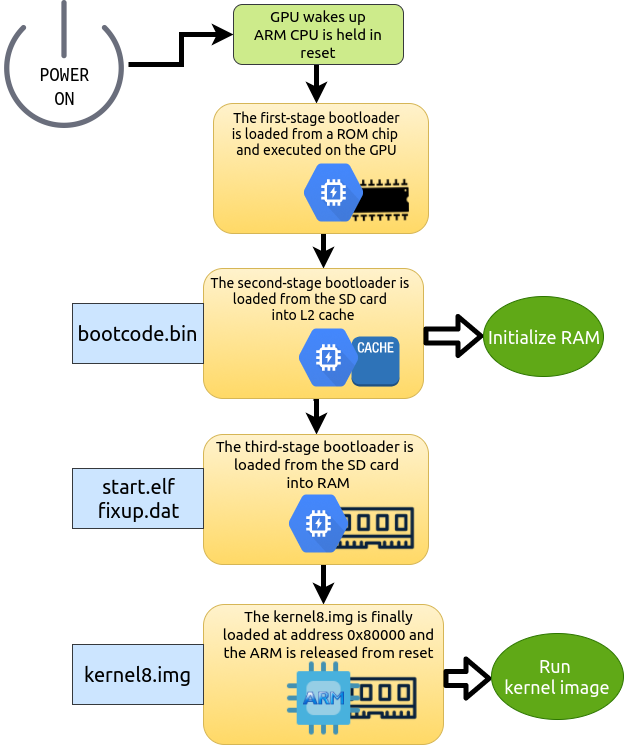
\includegraphics[scale=0.6234]{tesi1.png}
 \caption[Figure 1]{Explanatory diagram on BMC2837 boot sequence}\label{fig:prima}
 \end{figure}
 \clearpage
%TODO: add a diagram

Every step up until the loading of the kernel image in memory is handled by 
the GPU and can be safely ignored after an initial setup.

\subsection{MicroSD Contents}
The microSD must have its first partition formatted as FAT32; there are no 
further restrictions on following partitions. The absolute bare minimum contents 
are just four files:
\begin{enumerate}
    \item \textbf{bootcode.bin}: second-stage bootloader, necessary for the GPU
            to load the third-stage bootloader.
    \item \textbf{start.elf}: third-stage bootloader, necessary for the GPU to load
            the kernel image in RAM.
    \item \textbf{fixup.dat}: a file containing relocation data to be referenced 
            by start.elf when loading into RAM; This allows for the same firmware 
            to be used for all versions of the Raspberry Pi, which range in 
            memory from 256MB to 1GB. If not included the board might still boot,
            but it will likely only report a total of 256MB regardless of the
            actual installed RAM.
    \item \textbf{kernel8.img}: kernel binary for the ARM CPU.
\end{enumerate}
Of those four files only the kernel image is user provided; the remaining firmware
is distributed and updated in compiled form by the Raspberry Pi foundation with
proprietary licensing from Broadcom.

\subsection{Configuration}
It is possible to configure in different ways the boot process by combining
different firmware binaries and config.txt options, but this work always uses
the default with no extra steps needed; this is to ensure the usage is kept
as simple as possible and since the base behaviour never presented any issue.
Of all the available options, only the following two were ever considered 
(but still never implemented).

\subsubsection{Architecture}
The Cortex A-53 can run both ARM32 and ARM64 code; the choice is dictated by the
name of the kernel image: {\tt kernel8.img} makes the CPU start in AArch64 mode,
while {\tt kernel7.img} would start in AArch32.

\subsubsection{Kernel Loading Address}
The GPU loads the kernel image starting at address 0x80000 in RAM for the
Raspberry Pi 3. By adding a config.txt file to the microSD card and using
the kernel\_address parameter the image file will be loaded at the specified
starting point. Similarly, by setting the kernel\_old parameter to 1 the binary
will be loaded at the beginning of the main memory, at address 0x0.

Although these options can bring a more clean memory disposition, it was decided
the advantages were not worth adding an additional file to the necessary setup.
Additionally, while the Raspberry Pi harware correctly interprets these commands
the Qemu emulated machine is not entirely loyal to reality and actively resists
any attempt to move the kernel to locations other than 0x80000 (more details can
be found in chapter 7).

\subsubsection{Memory Split}
As previously mentioned the two main actors on the BCM2837, the quadcode Cortex-A53 ARM
and the Videocore IV GPU, share the same 1GiB RAM space. Without other instruction
the start.elf bootloader fixes the separation at address 0x3C000000, keeping
64MiB to himself and leaving the rest to the CPU.

This split can be increased in favor of the GPU or minimized even further using
specific config.txt parameters. The only graphical feat required by this work
is the display of a simple framebuffer to present textual output; therefore
a reserved memory partition of 64MiB is more than sufficient.
It could be in fact reduced further to 16MiB, but as for the kernel load address 
adding the config.txt file was judged unneded effort on the user's side.

\section{Videocore IV}
After the control is passed to the ARM CPU it is never returned to the GPU.
The graphical processor however still has responsibility over some peripherals
and can carry on work under specific requests. The mean of communication 
between the two processing units is the shared RAM memory (and part of the interrupt
controller), specifically under the Mailbox interface.

\subsubsection{Mailboxes}
Mailboxes are the primary means of communication between the ARM and the 
Videocore firmware running on the GPU. A mailbox is nothing but a memory address
with special access modes tied to an interrupt signal for the receiving end.
Mailboxes consist of several 32 bit registers providing status information, read
and write access. If a value is written on right the memory location and the
mailbox is ready to accept data, an interrupt will be fired and the receiver
will have the chance to read the message and act accordingly. The data is 
usually another memory location, containing more elaborate commands and parameters.

Regarding the CPU-to-GPU mailbox, additional care must be taken to check whether
the mailbox is full or empty by inspecting the two most significant bits of 
the status register.

The data address to be written on the mailbox must be 16 bytes aligned in memory,
as the lowest 4 bits must be overwritten with the so called mailbox channel
number, a parameter detailing the nature of the request. As of time of writing
only two channels are defined: channel 8 for requests from ARM to the Videocore
and channel 9 for requests from the Videocore to the ARM. Apparently, channel 9
exists but has no definied behaviour.

The buffer whose address is written on the mailbox must contain properly structured
data for specific requests. Some of the possible commands from the ARM to the
Videocore include:
\begin{itemize}
    \item Get Broadcom firmware revision number.
    \item Get board model and revision number.
    \item Get board MAC address.
    \item Get current CPU-GPU memory split.
    \item Get or set power state for all the devices on the board.
    \item Get or set clock state for all the devices on the board.
    \item Get on board temperature readings.
    \item Control special GPIOs, like the on board activity led.
    \item Execute code on the Videocore.
    \item Require and manage a framebuffer to be displayed over the HDMI.
\end{itemize}

\subsubsection{Framebuffer}
The HDMI controller is managed entirely by the GPU, and the ARM core has no 
way to interact with it directly. Instead, it can ask through the mailbox
property channel for the Videocore to set up a framebuffer in its own memory
share and directly access it. The Videocore will then proceed to continously flush the
framebuffer's contents on the screen.
This is a very convenient design choice, removing a great deal of effor from
the OS developer to see output displayed on screen.


\section{Peripherals}
What follows is a list of all the peripherals used in the project with the core
functioning (registers and command codes) explained for each of them.
Device peripherals are connected to the ARM CPU through memory mapped I/O (MMIO);
their registers and buses are mapped in RAM starting from address 0x3F000000,
as if the main memory of the system extended beyond 1GiB.

\subsection{GPIO}

\subsection{External Mass Media Controller}

\subsection{UART Serial Interface}
There are two UART serial peripherals on board of the BCM2837: UART0 and UART1.
They can both be connected to the same group of six GPIOs to relocate the 
transmit and receive line; however, of those six pins only two (GPIO 14 and 15)
are externally accessible on the Raspberry Pi. This means that, at any time,
either of those pins can be connected and work for only one of the two serial
interfaces.
Even if this is undoubtedly a limitation it can pose an interesting
concurrency programming challenge for a student, as both can run successfully if 
properly alternated.

Those devices bear a strong similarity to $\mu$MPS' terminal devices, both having 
similar registers to check the current status and read or write character on the
interface. For this reason, except for the initialization of the peripheral
which is done entirely by the harware abstraction layer, they are left essentially
 untouched to be managed by students approaching the project. In comparison to 
 the emulated devices the only real difficulty lies in a less organized register
 structure, having about four registers scattered over a larger memory area instead
 of a compact structure; after providing a focused and complete documentation of 
 said registers, this complication should be easily overcome.

 \begin{figure}[t]
 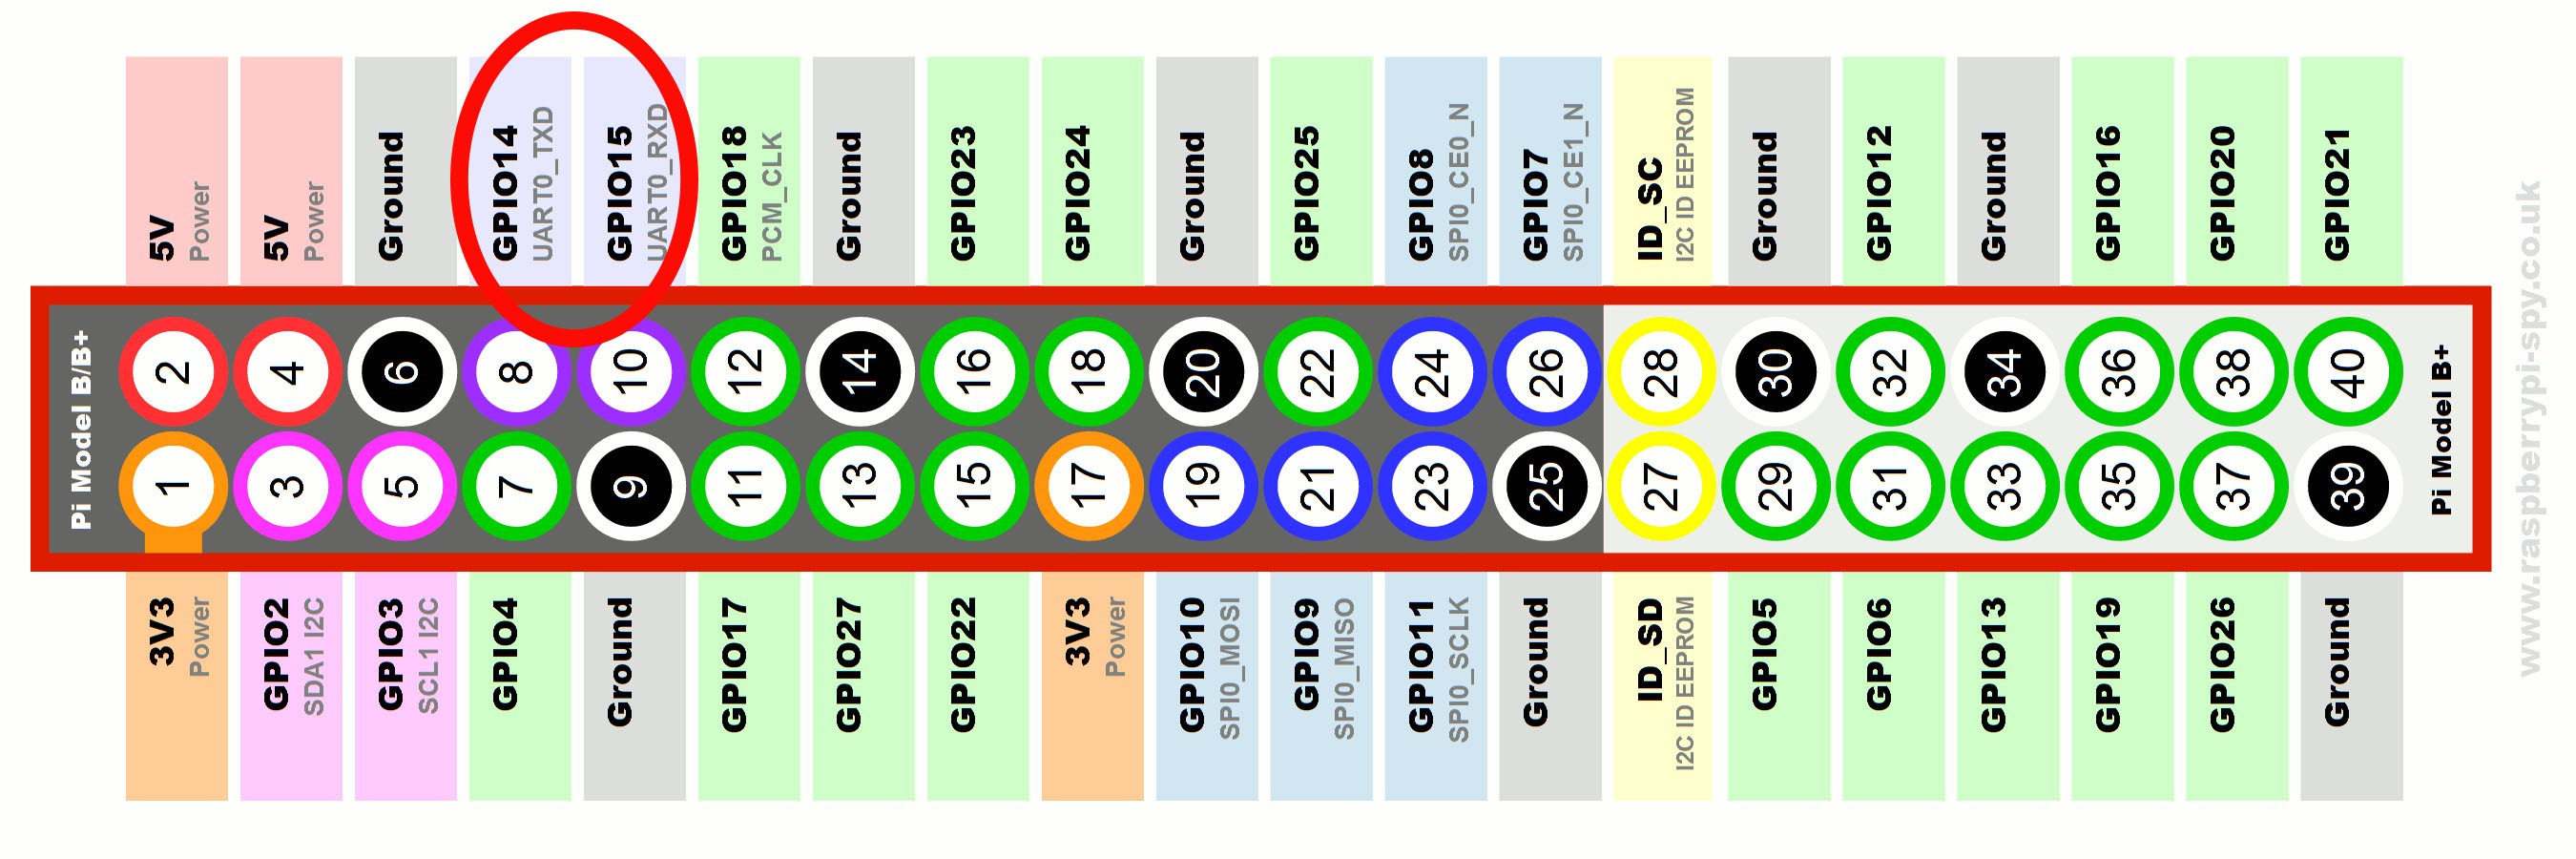
\includegraphics[scale=0.143]{tesi2.jpg}
 \caption[Figure 2]{Highlight of UART reserved GPIOs}\label{fig:seconda}
 \end{figure}

\subsubsection{UART0}
The UART0 is a fully fledged asynchronous serial interface, abiding to the 
PL011 ARM specification \cite{pl011}. To properly run on real hardware, the
corresponding pins must be configured to use the alternate function number 0 with
no internal pull up or down.
Its register are located starting at the address 0x3F201000, each of them
is 32 bits wide and they are organized as follows (some unimportant ones are omitted for brevity):
\begin{description}
    \item[Data:] this register contains the first character present in 
            the receive FIFO and can be written to send an outgoing character to 
            the transmit FIFO. Addidionally, it presents an error report of the ongoing
            connection, with a specific bit for every condition (overrun, break,
            parity, framing).
    \item[RSRECR:] a redundant register for error conditions.
    \item[Flag:] contains various flags on the current state of the UART, like 
            state (full or empty) of the transmit and receive FIFOs and whether
            the UART device is busy or idle.
    \item[IBRD:] integer part of the baudrate divisor: when configuring the device
            the baudrate is established as a floating point divisor prescaling
            the system clock. This is the integer part.
    \item[FBRD:] Floating point part of the baudrate divisor.
    \item[Line control:] this register manages configuration options like
            parity, number of stop bits, word length and FIFO abilitation.
    \item[Control:] this register controls the actual peripheral; mainly used
            for enabling and disabling the whole device.
    \item[IFLS:] interrupt FIFO level selection register. It is used to establish 
            at which percentage each FIFO (transmit or receive) triggers the
            corresponding interrupt. Possible values range from 1/8 to 7/8.
    \item[Interrupt mask:] allows to mask specific interrupts tied to the peripheral,
            such as those fired on reception and transmission of a character
    \item[Raw interrupt:] read only register updated with currently pending
            interrupts, regardless of the mask settings.
    \item[Masked interrupt:] same as the raw interrupt register but with the
            masked interrupt lines excluded.
    \item[Interrupt clear:] register to be written to clear pending interrupts.
\end{description}

Of all those registers, the only ones a student should really care about are
data, flag, interrupt mask, masked interrupt and interrupt clear. All the others 
are used for the initialization of the peripheral, which is handled by the 
hardware abstraction layer and should not be changed.

The serial interface is configured as 8 bit wide, no parity bit and with
a baudrate of 115200. The FIFOs are disabled for simplicity, so they act like 
a one character deep buffer.

\subsubsection{UART1 or Mini UART}
The UART1 is part of the group of auxiliary peripherals, together with two SPI
interfaces. In comparison with UART0 it has much more restricted functionality,
but still enough for a simple educational project. For example, it does not 
provide framing error detection or parity bit management, features that are either
disabled or ignored even in its more complete counterpart.
To properly run on real harware, the corresponding pins must be set to use the
alternate function number 5 with no internal pull up or down.
Its registers are located starting at the address 0x3F215040, each of them is 32 bits
wide and they are organized as follows (some unimportant ones are omitted for brevity):

\begin{description}
    \item[IO:] reading from this register yield the first character present in the
            receive FIFO, while writing it inserts the data into the write FIFO.
    \item[IIR:] register for enabling receive and transmit interrupts. If the first
            bit is set an interrupt line is asserted whenever the transmission FIFO
            is empty; if the second bit is set an interrupt line is asserted whenever
            the reception FIFO is not empty.
    \item[IER:] register holding information about which interrupt is pending (if any).
    \item[LCR:] controls whether the Mini UART works in 8 bit or 7 bit mode.
    \item[LSR:] line control status; used to determine if the device is ready to 
            accept new data or if there are received characters to be read.
    \item[CNTL:] control register to enable (in a separate fashion if so requested)
            the receive and trasmit lines.
    \item[BAUD:] 16 bit baudrate counter, to be set directly to the desired value.
\end{description}
Again, since the abstraction layer takes care of the initialization procedure
the user should really care about four registers: IO, IIR, IER and LSR.
The serial configuration is the same as the UART0.

\section{Interrupt Controller}
The BCM2837 SoC has at least two devices acting as interrupt controllers. One of 
them is clearly defined in the peripheral datasheet \cite{bcm2835}, while the
other is not clearly named but hinted at thorugh register definition in a later 
revision \cite{rev3.4}. Those are here arbitrarely named Base Interrupt Controller (BIC)
and Generic Interrupt Controller (GIC).
These two interrupt controllers are cascaded, meaning that 64 interrupt lines are 
wired to the BIC which in turn compresses them into 2 interrupt lines for the GIC
controller; additionally, the GIC also receives some interrupt lines from mailboxes
and USB.

 \begin{figure}[h]
 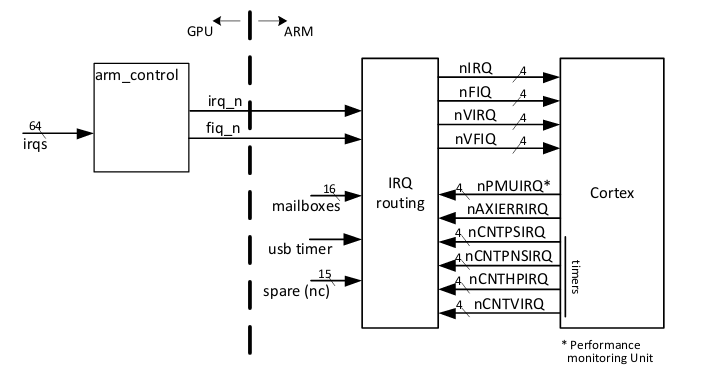
\includegraphics[scale=0.55]{tesi3.png}
 \caption[Figure 3]{BCM2837 interrupt controllers configuration}\label{fig:interrupt}
 \end{figure}
From a practical standpoint there are often serveral registers indicating which interrupt
line is being asserted at any moment. There is no apparent drawback in ignoring most
of them and just reading each device-specific register to discern which source fired
the exception.
The general interrupt organization is very confused and obscure. Interrupt functionality
was achieved mainly through examples and reverse engineering regarding the specific
device taken in consideration at the time.
What follows is a brief listing of interrupt related configuration for the devices
used in this work.

\begin{description}
    \item[UART] Both UART devices are cascated through the two interrupt controllers;
        although they can be checked via registers in both controllers, it is suggested
        to only read the Masked IRQ and IIR registers of the respective peripheral.
    \item[ARM timer] Being this an interrupt internal to the ARM processor its
        status has only been checked against the innermost interrupt controller (GIC).
        It is not clear whether it is present in the BIC as well.
    \item[Inter processor mailboxes] Possibly the sole source clearly
        depicted from the documentation, its presence can be understood from the 
        corresponding register in the Generic Interrupt Controller (as indicated
        by \ref{fig:interrupt}).
\end{description}

\subsection{Inter Processor Interrupt (IPI)}
In a multicore system such as the Raspberry Pi 3 the need arises for a privileged
communication channel between each core. The ARM Cortex-A53 does not provide an 
explicit method to do so, and it is left to the Generic Interrupt Controller to 
provide.
Similarly to the interface between ARM and Videocore there are mailboxes between
the four cores of the CPU as well.

The operation of those inter core mailboxes is much more straightforward than the
CPU-GPU counterpart. There are four for each core and for each mailbox the GIC
exposes three types control registers, for a total of 36 registers 
\footnote{Note: the first kind of register cover all four mailboxes for each core}.
\begin{description}
    \item[Mailbox Control] four registers of this type in total, one for each core
        and covering its four mailboxes. They enable an interrupt or fast interrupt
        line for each mailbox.
    \item[Mailbox Write-Set] four registers for each mailbox in every core, so 
        sixteen of them in total. They are write only and are used to put the
        actual data in the mailbox. Upon write the corresponding enabled exception
        (if any) is fired for the selected core.
    \item[Mailbox Read and Write-Clear] one register for each corresponding
        Write-Set register. They can be read to receive the data sent by writing
        in the Write-Set register, and have to be written to disarm the interrupt
        line. Each bit of the register is independent in firing the interrupt, so 
        to completely clear the same content that was read from the register must
        be written back on it.
\end{description}

\clearpage{\pagestyle{empty}\cleardoublepage}
\chapter{Emulated peripherals}

\clearpage{\pagestyle{empty}\cleardoublepage}
\chapter{Student's Perspective}

\clearpage{\pagestyle{empty}\cleardoublepage}
\chapter{Usage and Debugging}
\section{Final Result}
The final result of this work consists, from the user perspective, solely of 
two files: {\tt hal.elf} and {\tt hal.ld}.
The first is the the hardware abstraction layer compiled for an ARM64 target, 
containing system initialization and emulated devices management; the second is 
its linker script, to be used to link an application to the hal.

The hal performs all the necessary routines and then calls a {\tt main} function.
There is a weak-defined {\tt main} included with the hal that just echoes every
character received on UART0.
From there, the user provided code is expected to write specific memory addresses
to define new exception handlers and control emulated devices. 

One of the objectives of this work was to avoid creating ad hoc software and
relying as much as possible on widespread tools. Because of this, there is no
custom package like the $\mu$MPS2 emulator to install; instead the user needs
a proper cross compile toolchain for ARM64 (or an ARM64 device, like the Raspberry
Pi itself) and eventually Qemu.

Given a compiled elf with the user's code called {\tt app.elf} and assuming to
use {\tt aarch64-elf-gcc} as a cross compiler, the process to create a kernel image
would be 
\begin{lstlisting}
aarch64-elf-ld -nostdlib -nostartfiles -Thal.ld \
    -ooutput.elf hal.elf app.elf                                                                                                                                    
aarch64-elf-objcopy output.elf -O binary kernel8.img
\end{lstlisting}
The resulting binary can then be placed on a microSD card and run on a Raspberry Pi 3
or on Qemu

\section{Qemu}
Since version 2.12 Qemu supports a Raspberry Pi 3 emulated machine.
The official version for the Linux distro of choice may be less recent, in 
which case the user needs to compile the package from source.
 Particular care was taken in assuring the same code runs with no discernible difference on
the emulator and the device, which was not a difficult task.
Usually, in the rare situations where virtual and real boards differ in their
behaviour the real hardware is in the right (as one would expect).
Some examples found along the way are:
\begin{itemize}
    \item Uninitialized memory location will inevitably contain null values if 
        running under Qemu; the real world RAM is not so clement, and will live 
        up to the tale of having its content randomized after a reset.
    \item The MMU memory configuration includes distinguishing between device
        and normal memory: while the latter ban be subject to caching to increase performance,
        the former will not be optimized. Device memory is meant for memory mapped
        areas that are connected to peripherals, as their volatile nature would
        mix with caching for uncoherent results.
        Failing to set the device area as device memory will be forgiven on Qemu
        as there are no real peripherals; instead, the Raspberry Pi board will most likely
        not behave as expected.
    \item Qemu is whimsical about the memory address where to load the kernel image.
        The emulator's boot sequence is different from the real device as the
        {\tt kernel8.img} file is not read from the microSD card but passed from
        the command line. Qemu invariably starts the execution by jumping at 
        {\tt 0x80000}; if that is not the same address referenced by the linker
        script the kernel will fail to run.
\end{itemize}

Qemu requires a kernel image and a microSD card image to be passed as command
line arguments. An example command to run the emulator is:
%TODO: specify how to create an image
\begin{lstlisting}
qemu-system-aarch64 -M raspi3 -kernel kernel8.img \
    -drive file=drive.dd,if=sd,format=raw \
    -serial vc -serial vc
\end{lstlisting}

Where the command line options have the following meaning:
\begin{description}
    \item[-M raspi3] specifies the machine to emulate.
    \item[-kernel kernel8.img] specifies the kernel image to run.
    \item[-drive file=drive.dd,if=sd,format=raw] attaches the microSD card, here
        using an image file. Note that a real device can be used in the same way,
        for example using {\tt file=/dev/mmcblk0}, allowing to run both on the
        board and the emulator with the same exact drive.
    \item[-serial vc] each serial option accounts for a UART interface (UART0 and UART1,
        in this order). {\tt vc} stands for ``virtual console'' and will open a 
        tab in the Qemu window. Another possible value is {\tt stdio}, which will
        conveniently pipe the serial output of the chosen interface on the shell
        (obviously available for only one of the two UARTs).
\end{description}

\section{Debugging}
The debug of the compiled kernel can be carried over Qemu with GDB. Using the
{\tt -gdb tcp:1234} parameter Qemu opens a debugging tcp port for a GDB client
to connect to (another port can be specified). The {\tt -s} command line flag 
brings the same result in a shorter format, and by adding {\tt -S} as well the
emulator will not start the execution, allowing the developer to connect.

Once the emulator is ready, a GDB client can connect to it. A client for
ARM64 should be present within the toolchain used to compile the kernel.
 A simple command line client may attach using the following commands (assuming
 the {\tt aarch64-elf-gcc} toolchain is installed)

\begin{lstlisting}
aarch64-elf-gdb
file output.elf
target remote localhost:1234
\end{lstlisting}

Emulators like $\mu$MPS2 have the prominent advantage of a specifically designed
running and debugging interface; nonetheless, a GDB server is a complete and
advanced debugging suite. The command line debugger may seem a scarce alternative,
but there are plenty of richer options; the author recommends {\tt gdbgui}, 
a browser-based Python GDB client.
Gdbgui can be installed via {\tt pip} or as an official package. It must be launched
with the {\tt --gdb} (or {\tt -g}) command line option to specify a proper GDB
client (i.e. the one found within the ARM64 toochain); it acts as a web server
reachable at the default port {\tt 5000} with any browser, and provides an intuitive
interface fitted with step-by-step debugging, memory inspection, threaded view and
so on.

 \begin{figure}[t]
 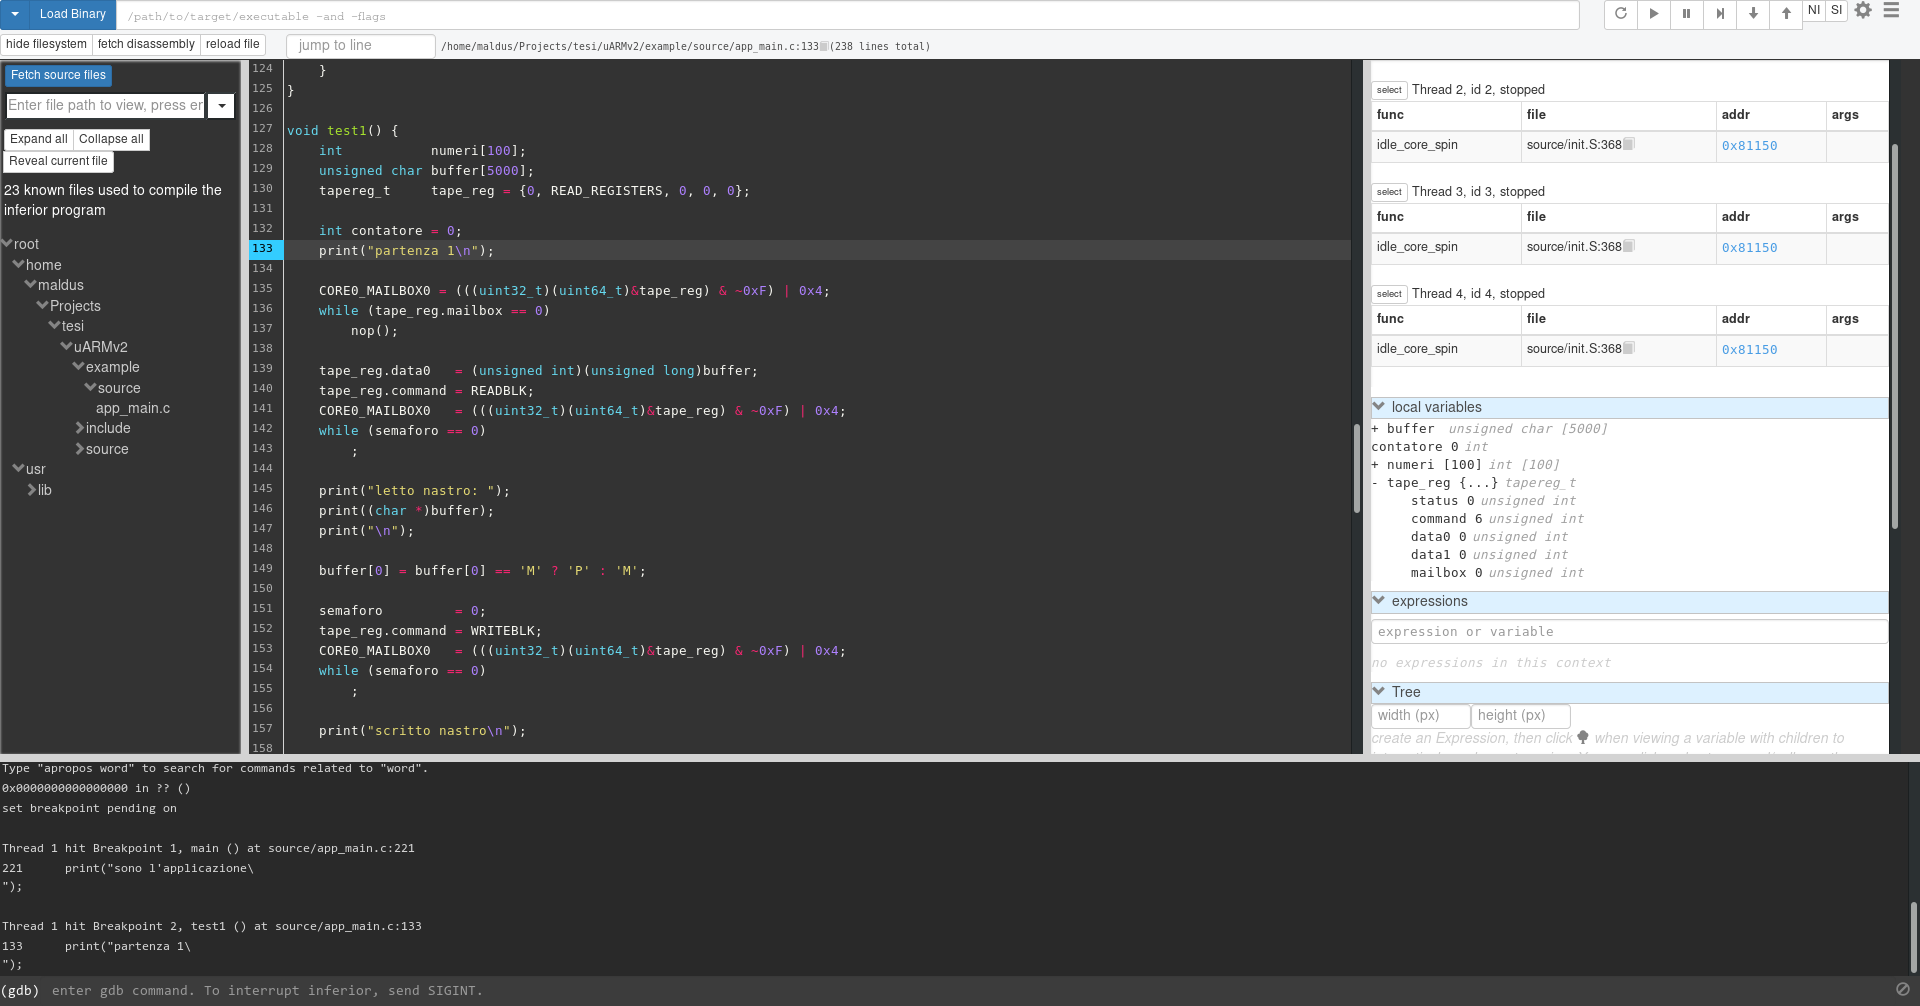
\includegraphics[scale=0.34,angle=-90,origin=c]{tesi4.png}
 \caption[Figure 4]{gdbgui browser interface}\label{fig:gdbgui}
 \end{figure}





%%%%%%%%%%%%%%%%%%%%%%%%%%%%%%%%%%%%%%%%%non numera l'ultima pagina sinistra
\clearpage{\pagestyle{empty}\cleardoublepage}
%%%%%%%%%%%%%%%%%%%%%%%%%%%%%%%%%%%%%%%%%per fare le conclusioni
\chapter{Conclusions and Future Work}
\section{Debugging with GDB}
Being a off-the-shelf software GDB is flexible enough to be extended with 
a specifically tailored client. GDB provides a machine interpreter that recognizes
machine readable commands for the purpose of creating higher level interfaces.

If the generic approach of gdbgui was deemed too complex for inexperienced graduate
students one could implement a $\mu$MPS2-like debugging interface that connects
to the Qemu GDB server. Using the same interface but on a different note a
debugging environment could be created inside a commonly used IDE, like Atom or 
Visual Studio Code.

\section{Other ARM64 SoC}
Although it is now firmly seated in the Olympus of open source educational boards,
the Raspberry Pi family is build on awfully obscured and undocumented hardware.
Broadcom follows the market trend of not releasing any information on its 
products like other manufacturers.
There are many Raspberry Pi-like boards that base themselves on similar hardware:
namely, a potent ARM CPU assisted by a graphical processing unit. In principle,
the work that has been done for the British board could be easily ported to a 
wide number of similar devices. The Pine64 family, for example, has recently
marketed a laptop powered by one of their compute modules. Running a toy
OS on a real laptop could be a even higher highlight for an undergraduate
or even graduate student.

\begin{thebibliography}{90}             %crea l'ambiente bibliografia
\addcontentsline{toc}{chapter}{Bibliography}
%%%%%%%%%%%%%%%%%%%%%%%%%%%%%%%%%%%%%%%%%provare anche questo comando:
%%%%%%%%%%%\addcontentsline{toc}{chapter}{\numberline{}{Bibliografia}}
\bibitem{minix} Andrew S. Woodhull, Andrew S. Tanenbaum, 
                Operating System Design and Implementation, 1997.
\bibitem{bakingpi} University of Cambridge, Department of Computer Science and Technology,
                    Baking Pi - Operating Systems Development,
                    \url{https://www.cl.cam.ac.uk/projects/raspberrypi/tutorials/os/}
\bibitem{davolimorsiani} M. Goldweber, R. Davoli, and M. Morsiani,
                        \"The Kaya OS project and the $\mu$MPS hardware emulator\",
                          SIGCSE Bull., vol. 37, pp. 49-53, June 2005.
\bibitem{tesijonjic} T. Jonjic,
                    \"Design and Implementation of the $\mu$MPS2 Educational Emulator\",
                    Alma Mater Studiorum, 2012.
\bibitem{tesimelletti} M. Melletti,
                    \"Studio e Realizzazione dell'emulatore $\mu$ARM e del progetto
                    JaeOS per la Didattica dei Sistemi Operativi\",
                    Alma Mater Studiorum, 2016.
\bibitem{ultibo} The Ultibo Project, \url{https://ultibo.org/}
\bibitem{circle} The Circle C++ environment, \url{https://github.com/rsta2/circle}
\bibitem{bcm2835} BCM2835 ARM Peripherals, Broadcom.
\bibitem{rev3.4} ARM Quad A7 Core, Broadcom.
\bibitem{pl011} PrimeCell UART (PL011) Technical Reference Manual, ARM.
\end{thebibliography}
%%%%%%%%%%%%%%%%%%%%%%%%%%%%%%%%%%%%%%%%%non numera l'ultima pagina sinistra
\clearpage{\pagestyle{empty}\cleardoublepage}
\chapter*{Ringraziamenti}
\thispagestyle{empty}
Qui possiamo ringraziare il mondo intero!!!!!!!!!!\\
Ovviamente solo se uno vuole, non \`e obbligatorio.
\end{document}
